\section{Neural Networks}
\subsection{Why Neural Networks?}
Neural networks are needed to resolve the limitations of other seen models. More in depth:
\begin{itemize}
    \item \textbf{Perceptron:} can only learn linearly separable functions;
    \item \textbf{Kernel Machines:} add the concept of non-linearity, but the choice of the appropriate kernel is not trivial;
\end{itemize}
\subsection{Multi Layer Perceptron}
A Multi Layer Perceptron (MLP) is a network of interconnected neurons, organized in layers. Neuorns from one layer
sends their output to the neurons of the next layer. The first layer is called \textit{input layer}, one or mode \textit{hidden layers}
are in the middle, and the last layer is called \textit{output layer}.

\begin{tikzpicture}[
    node distance=12mm,
    every node/.style={draw,circle,minimum size=8mm},
    input/.style={fill=purple!50},
    hidden/.style={fill=green!20},
    output/.style={fill=red!50},
    arrow/.style={-{Latex[length=2mm]},thin}
]

% INPUT LAYER
\node[input] (i1) at (0,0)  {};
\node[input] (i2) at (1.2,0) {};
\node[input] (i3) at (2.4,0) {};
\node[input] (i4) at (3.6,0) {};
\node[input] (i5) at (4.8,0) {};
\node[draw=none] at (2.4,-1) {$x$};
\node[draw=none] at (-1.3,0) {Input layer};

% LAYER 1 (3 nodes)
\node[hidden] (h11) at (1.0,1.5)  {};
\node[hidden] (h12) at (2.4,1.5)  {};
\node[hidden] (h13) at (3.8,1.5)  {};
\node[draw=none] at (-1.3,1.5) {Layer 1};

% LAYER 2 (3 nodes)
\node[hidden] (h21) at (1.0,3.0)  {};
\node[hidden] (h22) at (2.4,3.0)  {};
\node[hidden] (h23) at (3.8,3.0)  {};
\node[draw=none] at (-1.3,3.0) {Layer 2};

% LAYER 3 (unchanged)
\node[hidden] (h31) at (1.2,4.5)  {};
\node[hidden] (h32) at (2.4,4.5)  {};
\node[hidden] (h33) at (3.6,4.5)  {};
\node[draw=none] at (-1.3,4.5) {Layer 3};

% OUTPUT LAYER
\node[output] (o1) at (2.4,6.0) {};
\node[draw=none] at (-1.3,6.0) {Output layer};

% Connections
\foreach \i in {1,...,5}{
   \foreach \h in {11,12,13}{
     \draw[arrow] (i\i) -- (h\h);
   }
}
\foreach \a in {11,12,13}{
   \foreach \b in {21,22,23}{
     \draw[arrow] (h\a) -- (h\b);
   }
}
\foreach \a in {21,22,23}{
   \foreach \b in {31,32,33}{
     \draw[arrow] (h\a) -- (h\b);
   }
}
\foreach \a in {31,32,33}{
     \draw[arrow] (h\a) -- (o1);
}

% Equations on the right
\node[draw=none,anchor=west,text width=7cm] at (6,4.5)
  {$\phi_3(x)=\sigma(W_3\phi_2(x))=\sigma(W_3\sigma(W_2\sigma(W_1 x)))$};
\node[draw=none,anchor=west,text width=7cm] at (6,3.0)
  {$\phi_2(x)=\sigma(W_2\phi_1(x))=\sigma(W_2\sigma(W_1 x))$};
\node[draw=none,anchor=west,text width=7cm] at (6,1.5)
  {$\phi_1(x)=\sigma(W_1 x)$};
\node[draw=none,anchor=west,text width=7cm] at (6,6.0)
  {$f(x)=w^\top \phi_3(x)$};
\end{tikzpicture}

Where:
\begin{itemize}
    \item $\boldsymbol{x}$ is the input vector;
    \item $\phi_i(x)$ is the output of layer $i$, learned from the data during training.
    \[\phi_i(x) = \sigma(W_i \boldsymbol{x})\]
    \item $W_i$ is the weight matrix of layer $i$. It's dimensions depend on the number of neurons in layer $i$. 
    Each row contains the weights associated to a neuron. Computing $W_i \boldsymbol{x}$ will return a vector
    which contains the weighted sum of the inputs for each neuron in layer $i$.
    \item $\sigma(\cdot)$ is a non-linear activation function, applied element-wise.
\end{itemize}
The final output is computed as a linear combination in the new feature space created by the hidden layers.
Differently from SVMs, where the kernel is chosen \textit{a priori}, in MLPs the transformation is learned from data. The only
downside is that training is requires more data and more computational power.
\subsubsection{Activation Functions}
Activation functions introduce non-linearity in the model. We will analyze some proposed functions:

\paragraph{Threshold activation:}
the treshold activation, already seen in the perceptron model, is defined as:
\[ f(\boldsymbol{x}) = sign(\boldsymbol{w}^T \boldsymbol{x}) \]
It's cannot be used in MLPs, since it's derivative is zero almost everywhere, apart from the discontinuity in zero (not differentiable). 
This makes impossible to use gradient-based optimization methods for training.

\paragraph{Sigmoid activation:}
The sigmoid activation function is defined as:
\[ f(\boldsymbol{x} = \sigma(\boldsymbol{w}^T \boldsymbol{x}) = \frac{1}{1 + e^{-\boldsymbol{w}^T \boldsymbol{x}}} \]
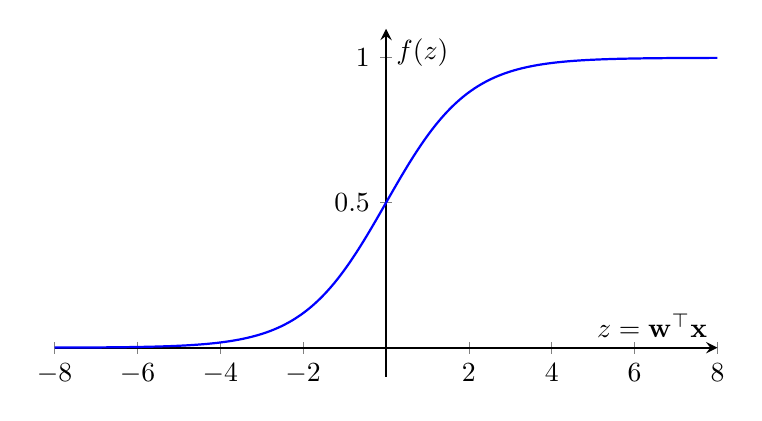
\begin{tikzpicture}
\begin{axis}[
    axis lines = middle,
    xlabel = {$z = \mathbf{w}^\top \mathbf{x}$},
    ylabel = {$f(z)$},
    ymin = -0.1, ymax = 1.1,
    samples = 200,
    domain = -8:8,
    width=10cm,
    height=6cm,
    thick,
]

\addplot[blue] {1/(1 + exp(-x))};
\end{axis}
\end{tikzpicture}
It represents a smooth approximation of the threshold function. It is approximately linear around zero, which helps in gradient-based optimization.
However, for large positive or negative values of $z$, the function saturates (approaches 0 or 1), causing the gradient to vanish.
\subsubsection{Output Layer}
The output layer of a neural network produces the final predictions. The function used can be 
different from the one used in hidden layers and heavily depends on the task at hand.
\\We will now analyze the activation functions used in the output layer for different tasks.
\paragraph{Binary Classification:} for binary classification tasks, only one output neuron $o(\boldsymbol{x})$ is needed.
The output activation function is usually the sigmoid activation function, which maps the output to the range (0, 1). It is defined as:
\[ f(\boldsymbol{x}) = \sigma(o(\boldsymbol{x})) = \frac{1}{1 + e^{-o(\boldsymbol{x})}} \]
This output can be interpreted as the probability of belonging to the positive class.
To obtain the final class label, a threshold (usually 0.5) is applied:
\[ y^* = sign(f(\boldsymbol{x}) - 0.5) \]

\paragraph{Multi-class Classification:} for multi-class classification, similar to what was done with single layer perceptrons, a one vs all approach can be used.
This requires $K$ output neurons, one for each class. The softmax activation function is commonly used in this case, defined as:
\[ f_i(\boldsymbol{x}) = \frac{e^{o_i(\boldsymbol{x})}}{\sum_{j=1}^{K} e^{o_j(\boldsymbol{x})}} \quad \text{for } i = 1, 2, \ldots, K \]
This function converts the raw output scores into probabilities that sum to 1 across all classes. This is not activated element-wise, but
it is a layer-wise activation function.
The predicted class is the one with the highest probability:
\[ y^* = \arg\max_{i} f_i(\boldsymbol{x}) \] 

\paragraph{Regression:} for regression tasks, where the output is a continuous value, the decision is the value of the output neuron itself.

\subsubsection{representational power of MLPs}
In this section we will analyze the representational power of MLPs on different tasks.
\begin{itemize}
    \item \textbf{Boolean functions:} any boolean function can be represented by a MLP with two layers of units. This can be done using CNF or DNF, but it would require
    an exponential number of hidden units in the worst case;
    \item \textbf{Continuous functions:} any bounded continuous function can be approximated arbitrarily well by a MLP with two layers of units (using sigmoid activations).
    \item \textbf{Arbitrary functions:} any function can be approximated arbitrarily well by a MLP with three layers of units (using sigmoid activations).
\end{itemize}

\subsection{Training Multi Layer Perceptrons}
Similarly to other models, MLPs are trained by minimizing a loss function on the training data. Different loss functions can be used depending on the task at hand.
\subsubsection{Loss Functions}
\paragraph{Binary Classification:}
For binary classification tasks, the binary cross-entropy loss is commonly used. It is defined as:
\[ L(y, f(\boldsymbol{x})) = - (y \log(f(\boldsymbol{x})) + (1 - y) \log(1 - f(\boldsymbol{x}))) \]
This can be interpreted as a switch function between two log-likelihoods, depending on the true label $y$. By putting the minus sign,
we convert the maximization problem into a minimization one (from a likelihood to a loss).

\paragraph{Multi-class Classification:}